\section{Overview of Language and System}
\label{sect:Overview}
In this section, we give an overview of the whole system architecture within which \rolang programs executed and then discuss key language features with an example.

We call an entity executing a \rolang program an {\em agent\/} or a {\em process.\/}
The hardware abstraction on which \rolang programs executes includes (a) a controller, (b) shared memory, in addition to the usual (c) local memory and processing unit of the agent.  
%
The controller receives lists of way-points and obstacles from the agent's program, drives the actuators (e.g. motors) to reach the way-points while avoiding the obstacles using sensors (e.g. GPS), and updates certain flags to indicate its status to the program.
%
The shared memory abstraction provides single-writer and multi-writer distributed shared variables using which an agent's program can communicate with another agent's program. 

%A \rolang program interacts with 
\begin{figure}[t!]
	\centering
	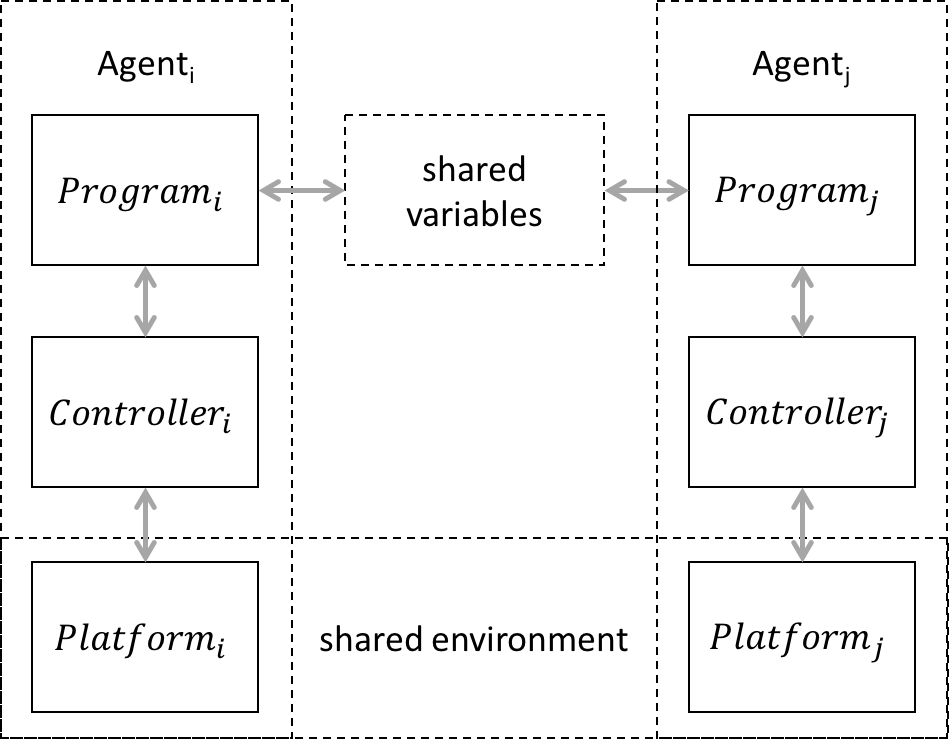
\includegraphics[scale=0.4]{figs/arch.png}
	\caption{\small Architecture of distributed system. Agent programs interact through shared variables. Each agent program also sets waypoints for its own controller which control the physical motion of the agent's platform. The agent platforms inhabit a shared physical environment, and therefore, also interact physically.}
\end{figure}

%\rolang allows users to write applications that will run on a distributed system of agents. 
For this paper, we assume that all agents execute the same \rolang program. A program is a collection of \emph{variable declarations} and \emph{events}. 
The language provides two types of shared variables:
(a) a {\em multi-writer} shared variable, declared in an \verb|allrw| block, allows all agents to read and write to the variable. 
(b) a {\em single-writer\/} shared variable, declared in the \verb|shared| 
% Resume here. 
single-writer} variables, which all agents can read from, but only one agent can write to. These variables are parameterized by the \verb|agent index|, an integer which is a unique identifier for each agent in the system, and they are declared in the \verb|SW| block. Local variables are declared in \verb|Loc|al declaration blocks.  \newline

As mentioned earlier, \rolang uses a \emph{precondition-effect} style of programming. These precondition and effect statements form events. Each application consists of a special \verb|Init| event, and an \verb|EventBlock|. The \verb|Init| event occurs at the beginning when the application starts executing, and it contains all statements which need to be executed only once; for instance, initializing a shared array. After the \verb|Init| event is executed, the \verb|EventBlock| starts executing. It contains a list of events that define the behavior of the application. The preconditions of each of the events inside the \verb|EventBlock| are evaluated in order of appearance, and the effect is executed if the precondition becomes true. The \verb|EventBlock| can be seen as a (potentially) infinite while-loop. 

We also provide an abstraction to manage the physical control of the agents, called \verb|doReach|, which takes as input a \emph{target} to reach, and a list of (predetermined) \emph{obstacles} which need to be avoided. We do not need to specify the format of the obstacles, as different implementations of this \verb|doReach| can have different specifications, but the target in general has the same type as the time varying variables of the system. \verb|doReach| communicates with the program using two flags, \emph{doReach_done}, and \emph{doReach_fail}. If the target is reached, the \emph{doReach_done} is set to true, and the \emph{doReach_fail} is set to true when the agent does not seem to have reached the target.

The next section presents the formal syntax, and an example to illustrate the structure of a general application. 

\subsection{Syntax}
\label{sect:syntax}
This section describes the formal syntax of \rolang. We first provide the major features of the formal syntax which describe program structure, event structure, and statement structure. 
\begin{figure}[ht!]
\footnotesize
\begin{center}
\noindent\begin{minipage}{.45\textwidth}
\begin{grammar}
<Pgm> :: <VarDecls><InitBlock><EventBlock>

<VarDecls> :: <MwDecls><SwDecls><LocDecls>

<MwDecls> :: "MW :" <Decls>

<SwDecls> :: "SW :" <Decls>

<LocDecls> :: "Loc :" <Decls>

<Decls> :: <Decl> <Decls> \\
         | <Empty>

<Decl> :: <EnumDecl> ";" \\
         | <ArrayDecl> ";" \\
         | <Type> <Var> ";"\\
         | <Type> <Var> "=" <Expr>
 
<InitBlock> :: "Init :" <Stmts>
\end{grammar}
\end{minipage}\hfill
\noindent\begin{minipage}{.45\textwidth}
\begin{grammar}
<EventBlock> :: "EventBlock:" <Events>

<Events> :: <Event><Events> | <Event>

<Event> :: <EventName> "(" <Expr> ")" "Pre" "(" <Expr>")" ";" "Eff :" <Stmts> 

<Stmts> :: <Stmt><Stmts> \\
		| <Empty>

<Stmt> :: <Assignment> \\
		| <If-Then-Else> \\
        | <Loop>\\
        | <Atomic>
		| <FunctionCall>
        
<Atomic> :: "Atomic :" Stmts
\end{grammar}
\end{minipage}
\end{center}
\caption{Language Syntax Features}
\end{figure}
As mentioned in the overview, each program consists of three major parts, with variable declarations, an initialization block and an event block. Aside from usual data types and arrays, we provide support for declaring enumerated types, as it is easy to use them as "stages" in applications.\footnote{https://github.com/ritwika314/RoLang/StarL/HLL/Examples/LeaderElect}

Events, as mentioned earlier are specified by precondition-effect blocks, where the precondition is a boolean expression, and effect blocks contain statements, which can be assignment statements, \verb|if-then-else| statements, \verb|Atomic| statements, function calls, or loops. We omit the productions for the more obvious syntactic elements like expressions, assignment statements, loops, etc.\footnote{https://github.com/ritwika314/RoLang/StarL/HLL/Semantics/agent-syntax.k}